%& C:\Users\glyph\AppData\Roaming\TikzEdt\TikzEdt\023~1.0\TEMP_H~1
\begin{document}
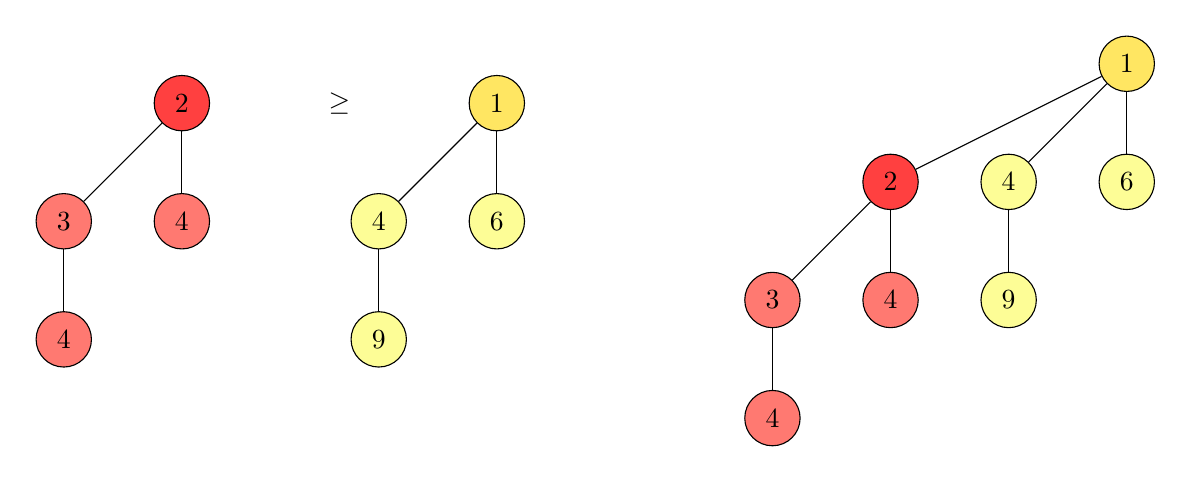
\begin{tikzpicture}
\definecolor{pastel-red}{HTML}{FF7971}
\definecolor{pastel-yellow}{HTML}{FDFD96}
\definecolor{sat-yellow}{HTML}{FFE662}
\definecolor{sat-red}{HTML}{FF4040}

\node [shape = circle, minimum size = 2em, draw = black, fill = sat-red] (v1) at (0,0) {$2$};
\node [shape = circle, minimum size = 2em, draw = black, fill = pastel-red] (v2) at (0,-1.5) {$4$};
\node [shape = circle, minimum size = 2em, draw = black, fill = pastel-red] (v3) at (-1.5,-1.5) {$3$};
\node [shape = circle, minimum size = 2em, draw = black, fill = pastel-red] (v4) at (-1.5,-3) {$4$};
\node [shape = circle, minimum size = 2em, draw = black, fill = sat-yellow] (v5) at (4,0) {$1$};
\node [shape = circle, minimum size = 2em, draw = black, fill = pastel-yellow] (v6) at (4,-1.5) {$6$};
\node [shape = circle, minimum size = 2em, draw = black, fill = pastel-yellow] (v7) at (2.5,-1.5) {$4$};
\node [shape = circle, minimum size = 2em, draw = black, fill = pastel-yellow] (v8) at (2.5,-3) {$9$};
\draw  (v1) edge (v2);
\draw  (v1) edge (v3);
\draw  (v3) edge (v4);
\draw  (v5) edge (v6);
\draw  (v5) edge (v7);
\draw  (v7) edge (v8);
\node at (2,0) {$\geq$};
\node at (6,-1.5) {$\implies$};


\node [shape = circle, minimum size = 2em, draw = black, fill = sat-red] (v21) at (9,-1) {$2$};
\node [shape = circle, minimum size = 2em, draw = black, fill = pastel-red] (v22) at (9,-2.5) {$4$};
\node [shape = circle, minimum size = 2em, draw = black, fill = pastel-red] (v23) at (7.5,-2.5) {$3$};
\node [shape = circle, minimum size = 2em, draw = black, fill = pastel-red] (v24) at (7.5,-4) {$4$};
\node [shape = circle, minimum size = 2em, draw = black, fill = sat-yellow] (v25) at (12,0.5) {$1$};
\node [shape = circle, minimum size = 2em, draw = black, fill = pastel-yellow] (v26) at (12,-1) {$6$};
\node [shape = circle, minimum size = 2em, draw = black, fill = pastel-yellow] (v27) at (10.5,-1) {$4$};
\node [shape = circle, minimum size = 2em, draw = black, fill = pastel-yellow] (v28) at (10.5,-2.5) {$9$};
\draw  (v25) edge (v26);
\draw  (v25) edge (v27);
\draw  (v27) edge (v28);
\draw  (v25) edge (v21);
\draw  (v21) edge (v22);
\draw  (v21) edge (v23);
\draw  (v24) edge (v23);

\usetikzlibrary{calc}
\pgftransformreset
\node[inner sep=0pt,outer sep=0pt,minimum size=0pt,line width=0pt,text width=0pt,text height=0pt] at (current bounding box) {};
%add border to avoid cropping by pdflibnet
\foreach \border in {0.1}
  \useasboundingbox (current bounding box.south west)+(-\border,-\border) rectangle (current bounding box.north east)+(\border,\border);
\newwrite\metadatafile
\immediate\openout\metadatafile=\jobname_BB.txt
\path
  let
    \p1=(current bounding box.south west),
    \p2=(current bounding box.north east)
  in
  node[inner sep=0pt,outer sep=0pt,minimum size=0pt,line width=0pt,text width=0pt,text height=0pt,draw=white] at (current bounding box) {
\immediate\write\metadatafile{\p1,\p2}
};
\immediate\closeout\metadatafile
\end{tikzpicture}

\end{document}
